\documentclass{sig-alternate}
\usepackage[utf8]{inputenc} 
%\usepackage[hidelinks]{hyperref}
%\usepackage[autostyle,french=guillemets,babel]{csquotes}
\usepackage{graphicx} % support the \includegraphics command and options
%\usepackage[backend=biber]{biblatex}
%\addbibresource{biblio.bib}
% \usepackage[parfill]{parskip} % Activate to begin paragraphs with an empty line rather than an indent
\usepackage{booktabs}
\usepackage{array}
\usepackage{paralist}
\usepackage{verbatim} 
\usepackage{amsfonts}
\usepackage{fancyhdr}
\usepackage{times}
\usepackage{url}
%\pagestyle{fancy} % options: empty , plain , fancy
%\renewcommand{\headrulewidth}{0pt} % customise the layout...
%\lhead{}\chead{}\rhead{}
%\lfoot{}\cfoot{\thepage}\rfoot{}

\hyphenation{he-terogeneous infra-structure lea-kage rea-lizing accep-table modula-rity tool-kits ho-rizontally me-chanisms}

\title{From Nested Virtualization Architecture \\To 2D Security Management for Distributed Clouds}

\author{
\numberofauthors{3}
\alignauthor
Alex Palesandro\\
\affaddr{Orange Labs, France}\\
\texttt{alex.palesandro@gmail.com}
\alignauthor
Aurélien Wailly\\
\affaddr{Orange Labs, France}\\
\texttt{aurelien.wailly@orange.com}
\alignauthor
Marc Lacoste\\
\affaddr{Orange Labs, France}
\texttt{marc.lacoste@orange.com}
}

\begin{document}
\maketitle

\abstract{
%Today, hypervisors have to find a complex trade-off between functionalities provided and security assurance. Those requirements are contrasting by design:
%adding new features will generally increases the LoC and consequently the attack surface. On the contrary, those code additions are required to properly fulfill market requests. 
%
%Nested virtualization is a technique capable to diversify hypervisor features. Exploiting an extra layer of virtualization, we will be able to decouple different requirements, avoiding the need to find delicate trade-off.
%
%In this paper, we will analyze the state of nested virtualization in modern hypervisor and evaulating the impact of utilization of microhypervisor to enforce a stronger security level.
%The problem of homogeneity over multiple IaaS providers is receiving considerable attention with the evolution toward nested virtualization. These new architectures unveil user-centric opportunities such as efficient resources management and VM migration. However the inherent drawbacks hinder its global adoption with a larger TCB and the complexity to monitor another virtualization layer. Thus, we argue that the promising architectural view of micro hypervisors approach is the key to the separation of hypervisor duties and reducing the attack surface.
%
%Furthermore, our architecture mushrooms commodity and micro hypervisors to leverage nested virtualization in terms of user-data privacy, modularity, TCB size and compatibility. These design principles are evaluated for each architecture configuration and compared to establish a reference security architecture. The resulting combination is built over common hypervisors empowered with micro hypervisors features. A reference implementation proven the architecture to be viable and will be extended to meet broader hypervisor scopes, enabling migration over heterogeneous cloud servers.
Distributed cloud computing is now moving user-centric. The pro-mise of this evolution is: (1) unified resource management across IaaS providers, e.g., live migration independent from hypervisor technology; (2) increased customizability to choose the hypervisor services needed to realize fully à la carte, self-service clouds. However, a reality check shows that major interoperability and security barriers must be lifted, and complex trade-offs be found between functionalities provided and security assurance.
Nested virtualization (NV) brings both a homogeneous interface for distributed hypervisor features and enhanced IaaS security, protecting VMs even in case of hypervisor compromise. However, practical NV adoption is still hindered by code additions to an already very large hypervisor TCB and by limited hardware support. New distributed IaaS architectures are therefore required.\\

In this paper, we argue that micro-hypervisor (MH) architectures are the key to overcome such NV limitations. 
From the previous challenges, we derive a set of design principles that a distributed IaaS architecture should satisfy. 
We compare possible architectural designs combining NV with micro-hypervisor features to find the best trade-off between user data privacy, modularity, TCB size, and compatibility with multiple platforms. 
We sketch how the resulting architecture may serve as a basis for 2D security management of a cloud of clouds: vertically, across layers for hardened IaaS security, and horizontally spanning cloud domains for end-to-end security.
}


%The resulting combination is built over common hypervisors empowered with micro hypervisors features. 
%
%rchitecture mushrooms commodity and micro hypervisors to leverage nested virtualization
%
%
%
%Furthermore, our architecture mushrooms commodity and micro hypervisors to leverage nested virtualization in terms of user-data privacy, modularity, TCB size and compatibility. These design principles are evaluated for each architecture configuration and compared to establish a reference security architecture. 
%
%enhance NV architecture next generation of distributed clouds security and interoperabiltiyi issues.
%
%
%failureverall, current NV architectures lack some of the dedicated features found in modern hypervisors and the impossibility to rely on a tiny TCB (violating principles DP3 and DP4).
%If the first one is currently being addressed by hypervisor developers, the second simply has not be achieved with modern hypervisors so far.
%
%ypervisors have to find a complex trade-off between functionalities provided and security assurance. Those requirements are contrasting by design:
%%adding new features will generally increases the LoC and consequently the attack surface. On the contrary, those code additions are required to properly fulfill market requests. 
%
%the inherent drawbacks hinder its global adoption with a larger TCB and the complexity to monitor another virtualization layer.
%
%First, independence from the provider resulting in lower infrastructure operation overheads, more rapid deployment of services, but also increased homogeneity the customer being free a particular hypervisor technology. Second, increased customizability, as the customer can choose which virtualized services (e.g., for security) may be deployed resulting in fully a la carte clouds. Third, new business opportunities, as SCs and their (virtual) apps might become new markets in the manner of ecosystems from the mobile computing world (e.g., iPhone, Android). 
%
%User-centric: de DCC
%vers plus d'homogeneity
%problemes 
%verticaux
%horizontaux.
%
%NV: solutions pour résoudre certains de ces problèmes.
%
%VErticaux: ...
%Horizontaux: ...
%
%Mais limites ... + ...
%New architectural solutions must be found.
%
%In this paper explore potential of micro-hypervisor architectures to enhance NV architecture next generation of distributed clouds security and interoperabiltiyi issues.
%
%We explore design principles properties.
%
%We compare architecutral solutions combining NV+MH to find the best trade off between ..., ???; ... meilleure approche.
%
%We sketch finally: how this type of architecture could enable to perform 2D supervision xl alyer x domain.

\section{Introduction}
\label{sec:intro}

%% Motivation
%Cloud computing platform are a solid reality nowadays. 
% Modern cloud platforms are able to provide elastic use of resources, optimizing their allocation to meet user needs. 
% la prochaine mutation majeure du cloud computing est celle du nuage hybride, qui fédère dans une même infrastructure nuages privés, publics, ou communautaires. L’intérêt est de s’affranchir d’un fournisseur de nuage dédié, ou de bénéficier de la sécurité d’un nuage privé, tout en profitant de la flexibilité d’un nuage public.
% User-centric...
% Cloud computing today is essentially still provider-centric (PC). The landscape is an increasing number of fiercely competing cloud service providers (CSP), operating multiple heterogeneous clouds. Each CSP offers its own, feature-rich offerings for customer VMs, with a great diversity of services in areas like security (e.g., system and network intrusion monitoring, firewalling, anti-malware, data security), resource management (e.g., elastic load balancing), or high availability (e.g., checkpointing/recovery). Such services usually come in the form of virtual appliances, often based on hypervisor support.
% A strong push has thus recently been made towards a user-centric (UC) vision of the cloud  It might be described as a paradigm change in delivering cloud resources (e.g., compute, storage). To lift the interoperability barrier,  a resource distribution plane, a.k.a. super-clouds (SCs) is introduced, spanning CSPs to decouple resource production (CSPs) from consumption (customers). To tackle the control challenge, this plane is also an extensibility layer, where each new stakeholder operating the distribution layer (a.k.a. SC provider) may provide its own services enabling the customer to deploy self-service, customizable clouds ranging from the SaaS to the full IaaS level. Technically, the idea is to split the cloud infrastructure into provider- and user-controlled domains or modules, several design alternatives being available such extensible hypervisors, flexible hypervisor management interface (dom0), or nested virtualization.
%This vision brings a number of benefits. First, independence from the provider resulting in lower infrastructure operation overheads, more rapid deployment of services, but also increased homogeneity the customer being free a particular hypervisor technology. Second, increased customizability, as the customer can choose which virtualized services (e.g., for security) may be deployed resulting in fully a la carte clouds. Third, new business opportunities, as SCs and their (virtual) apps might become new markets in the manner of ecosystems from the mobile computing world (e.g., iPhone, Android). 

\noindent \textit{Distributed cloud computing (DCC) }is now turning into a reality: modern hybrid cloud platforms enable to benefit seamlessly both from private cloud security and from public cloud flexibility. DCC is also moving user-centric: customers demand greater empowerment to deploy self-service clouds really adapted to their needs, and to move away from a provider-dominated landscape of highly heterogeneous closed platforms and its infamous vendor lock-in~\cite{CSA:TT}. 

% Mais pb:
% We classified problems related to DCC horizontally and vertically.
% %% Cclassification des problèmes: Specific problem considered
%The horizontal view gathers features related to interactions between IaaS stacks, such as live migrations. The vertical view addresses features close to the isolation of execution environment on the same physical machine. This classification provide a global coverage of problems to solve to deliver a secure, stable and robust architecture.
However, current \textit{distributed cloud infrastructures (DCI) }suffer from two sets of limitations. These may be broadly classified as \textit{horizontal} and \textit{vertical} challenges.
% Problèmes horizontaux: Mais Interop
%DCC does not handle heterogeneous infrastructures which secludes providers in non-evolving hardware.
%2)	Un manque de vision globale et de flexibilité dans la gestion de la sécurité. En cause : l'hétérogénéité forte des politiques et mécanismes entre nuages élémentaires et leur manque d’interopérabilité. Les plates-formes d’interopérabilité actuelles sont de plus trop monolithiques : elles dépendent fortement de la volonté des fournisseurs de nuages de déployer certains services, et ne conviendront donc pas à tous les types de clients.
% 
%Unfortunately, this vision suffers from a lack of homogeneity. Many of those services have not been deployed due to deficiencies in: (1) unified control; and (2) interoperability. Lack of control is visible through vendor lock-in: such services are so tightly coupled with the CSP and on its willingness to deploy them, with little leeway for the customer. Control is also severely limited by monolithic infrastructures (e.g., non-flexible hypervisors hiding hardware capabilities) preventing fine-grained cloud customization by the customer. Lack of interoperability is mainly due to heterogeneity of services, hypervisor-specific and thus not compatible across CSPs. Despite much efforts, standardization might be too slow or too partial to solve such issues, as both customers and providers might want features that are not in the standard.
%•	Lack of flexibility and control for overall security management: this refines the previous interoperability and control challenges for security. For interoperability, the problem comes from heterogeneity of security components and policies between CSPs and SCs. This has a strong security impact by introducing more vulnerabilities due to mismatching APIs. How also to manage interoperability and trust between SCs? For flexibility: how to clearly separate the infrastructure between UC and PC security management elements? how to make that frontier flexible to achieve a continuum between PC and UC security services? and how to define in that continuum security services that are flexibly composable with other types of services (e.g., replication, transactions)?
Horizontally, DCIs lack interoperability, mainly due to heterogeneity of IaaS services, hypervisor-specific and not compatible across providers. Control is also severely limited by monolithic infrastructures preventing fine-grained cloud customization by users. 
% Problèmes verticaux: Securite
%Also, security remains the last hurdle toward wide adoption of DCIs. The user data are no more self contained but distributed among all parties without any proof of confidentiality, integrity or availability.
% 1)	Un manque de sécurité global. Dans chaque nuage élémentaire formant le nuage hybride, chaque couche logicielle (machines virtuelles, hyperviseur) s'avère extrêmement vulnérable aux attaques, rendant difficile une protection intégrée forte.
% •	Security vulnerabilities in infrastructure layers:  For instance, the hypervisor and its over-privileged dom0 is a target of choice for attackers due to its complexity. This makes difficult an integrated protection. How to place / coordinate counter-measures in those layers that usually are not aware of one another, each with their own monitoring mechanisms, while attacks span several layers? How also to continue to guarantee VM protection when one or several of those layers are compromised? 
Vertically, security remains the last hurdle toward wide adoption of DCIs. Due to their complexity, infrastructure layers remain extremely vulnerable to attacks, making it difficult to achieve strong isolation and integrated protection.

\newpage
%% La NV comme élément de réponse:
% As a first element of answer, the nested virtualization~\cite{turtle:ibm} performed a breakthrough with enhanced isolation capabilities on the same physical machine. The hypervisor is now virtualized by a thin layer~\cite{cloudvisor:zhang} to counter failures. Furthermore, the horizontal challenges were also included in this tiny layer to deliver an homogeneous interface for commodity hypervisors~\cite{art:blan, xclo:blank}. 
% Nested virtualization (NV) brings both a homogeneous interface for distributed hypervisor features and enhanced IaaS security, protecting VMs even in case of hypervisor compromise. 
% The hypervisor is now virtualized by a thin layer
Advances in \textit{nested virtualization (NV)} were a major step forward to tackle such challenges~\cite{turtle:ibm}. By virtualizing the hypervisor through a thin software layer, NV brings enhanced isolation capabilities on the same physical machine, protecting VMs even in case of hypervisor compromise~\cite{cloudvisor:zhang}. NV also provides a distributed homogeneous interface for commodity hypervisors~\cite{art:blan,xclo:blank}.
% Mais..
% - Mais limites...
% However these classic approaches suffers from several shortcomings detailed in Section~\ref{ref:challenges}. 
Practical NV adoption is still hindered by code additions to an already large hypervisor TCB (Trusted Computing Base) and by limited hardware support.  There is also currently no NV architecture solving both vertical and horizontal challenges simultaneously.
% - New architectural challenges are required...
New distributed IaaS architectures are therefore required.

%The previous works created both horizontal and vertical basic blocks from scratch. While being a necessary step, these approaches does not inherits the advances performed in terms of operating system security. The software architecture are mainly monolithic and yet-another-layer fends off security problems withoutfiguring them out. Our approach learns from security issues fixed by OS architecure~\cite{} and apply these patterns to leverage nested virtualization. In this paper we show that component-based architecures are a promising design for the next generation of clouds.

In this paper, we propose a new architectural approach for DCIs. We argue that advances in OS design bring significant improvements to traditional NV architectures: instead of relying on general-purpose hypervisors (GPHs) for both virtualization layers, new kernel designs allow to tackle more efficiently different sets of challenges separately in each layer. We make a position statement that \textit{micro-hypervisor (MH) architectures} combined with NV benefits are a promising design for the next generation of DCIs.

% Contributions.
%1)
%2)
%3)
This paper makes the following contributions. From previous challenges, we derive a set of design principles that a DCI architecture should satisfy. We compare possible architectural designs combining NV with MH features to find the best trade-off between user data privacy, modularity, TCB size, and compatibility with multiple platforms. We finally sketch how the resulting architecture may serve as basis for 2D security management of DCIs: vertically, across layers for hardened IaaS security, and horizontally spanning cloud domains for end-to-end security.
 %The first challenge means that threats will be both vertical, spanning layers, and horizontal, spanning domains  the SUPERCLOUD being a multi-layer, multi-domain distributed cloud infrastructure. Vertically, attacks currently target several infrastructure layers (e.g., VMs, hypervisor). Unfortunately, most existing defenses are generally for single layers only. This makes it difficult to grasp the overall extent of an attack. Horizontally, threats may propagate through the network from cloud to cloud. Unfortunately, most existing defenses are for single clouds only. Lack of interoperability in security policies and mechanisms is thus a major barrier to  unified hybrid cloud security. The second challenge means that although many defense mechanisms may be leveraged in this 2D landscape, they remain difficult to configure and to reconcile. The current “by hand” approach becomes a nightmare for security administrators. Despite some automated solutions for managing security of single clouds, there is currently no solution truly applicable to federations of clouds in practice.

This paper is organized as follows. Section~\ref{ref:challenges} presents the DCI challenges and design principles. Sections~\ref{sec:rw} and~\ref{sec:classic} review the NV ecosystem and analyze the limitations of traditional NV design. Section~\ref{sec:mh} presents the MH approach. Section~\ref{sec:archcomp} compares possible DCI architectures combining NV and MH according to the design principles.
Finally, Section~\ref{sec:arch} presents a preliminary DCI system architecture based on the best resulting design with promising properties for 2D management of DCI security.
%Furthermore, in Section 6 we define a security architecture for multi-cloud scenario, with an analysis of necessary software components to satisfy vertical design principles.
%In Section~\ref{sec:conclu}, we conclude the paper with future works and our vision of the SuperCloud.
% in section in section 6 we define a security architecture for multi-cloud scenario, with an analysis of necessary software components to satisfy vertical design principles. In section 8, we conclude the paper with future works in section 8.

\section{Challenges and Design Principles}
\label{ref:challenges}

\subsection{Challenges}

\noindent Deploying cloud applications able to transparently use resources of several heterogeneous platforms is still difficult. 
%The concept of super-cloud~\cite{art:blan, xclo:blank} tries notably to overcome such issues. 
Multi-platform coordination is hard, primarily due to lock-in to different standards. Unfortunately, such lock-in is not only due to market strategic decisions, but also reflects heterogeneity of virtualization technologies. For example, each cloud provider may use different storage systems or formats for VM images. Different hypervisors have today a low degree of compatibility between them. This generally hinders using some popular features like VM live migration across different platforms. Incompatibility is even greater considering each platform may adopt several types of virtualization techniques. This situation induces a tight dependency between the customer and the cloud provider. It may prevent guaranteeing service availability by relying on alternative providers, or setting up geographical optimizations according to cost or origin of traffic. This resulted in some dramatic data server failures in recent years, causing prolonged outage of service for many applications. We refer to this class of multi-platform issues as \textit{horizontal challenges}.

Several concerns were also raised about user data privacy and platform integrity. For users, preserving the privacy of their data stored on the cloud platform is important. However, due to overprivileged hypervisors, a curious or malicious administrator may easily retrieve such data~\cite{cloudvisor:zhang}. 
In a multi-tenant cloud, physical resource sharing between users may lead not only to VM data leakage but also to attacks against the IaaS~\cite{bot:att, sec:you}.
For the provider, a primary objective is thus to guarantee platform integrity. Unfortunately, commodity GPHs are not well adapted to observe deeply all layers of a running IaaS platform: running a GPH at the highest privilege level hampers detection and reaction on the hypervisor itself in presence of faulty or malicious behavior. Thus, both users and providers have a problem with overprivileged hypervisors.
%: the platform administrator cannot perform in-depth infrastructure monitoring nor can users concretely inspect administrator actions on their data. 
%A major challenge for new generations of DCIs will be to find acceptable trade-offs between such conflicting requirements. 
We refer to this class of layer-oriented issues as \textit{vertical challenges}.

\subsection{Design Principles}

\noindent We identified the following key DCI design principles to meet the previous challenges: 
%In what follows, those principles will serve as reading template to analyze different architectures.
\begin{itemize}[]
\item \textbf{DP1 User Data Privacy} An administrator (or another platform user) should not be authorized to inspect and analyze user data and VM instances without explicit user consent. A trade-off should be found to allow providers to detect and react to potential threats, but also to prevent unlimited platform and user data access by curious or malicious operators. Thus, a platform administrator should not manage the infrastructure directly using the highest privilege level. Instead, his actions on user data objects should be validated by a mutually-trusted kernel run in the most privileged mode. This kernel should also enforce memory page encryption to prevent snooping when pages are swapped out.
\item \textbf{DP2 Fail-Safe Modular Architecture} The architecture should be fail-safe, e.g., for automatically migration of VMs or user-data during an attack, or to recover from software failures. The number of safety-critical components should minimal to reach a low attack surface. The overall design should also be highly modular to enable platform reconfiguration.
\item \textbf{DP3 Small TCB} The number of vulnerabilities and failures in the platform is directly linked with the code size run at the highest privilege level. A small TCB architecture will improve safety and integrity by design.
\item \textbf{DP4 Inter-Platform Support} The cloud architecture should support different platforms and providers. The user VMs should run (and potentially be migrated) unmodified over different IaaS platforms.
\item \textbf{DP5 Compatibility with Legacy} Evolution in the IaaS architecture should avoiding disrupting existing third party applications. Platform interfaces should be kept as close as possible to existing ones to prevent code rewriting notably for applications.
\end{itemize}
In addition to the previous functional principles, another set of principles should be considered regarding effective feasibility of implementing the DCI architecture. For instance in terms of platform usability:
\begin{itemize}[]
\item \textbf{DP* Minimal Additional Code} Despite not being a strictly a technical limitation, the amount of code to be added and maintained to an existing architecture to meet functional requirements could become a show-stopper to its practical use.
\end{itemize}
In our analysis, we will consider not only the overall suitability of the architecture, but also the amount of effort needed to develop and deploy it. Table \ref{int:des} summarizes the previous principles and the class of challenges they address.
 
\begin{table}
\caption{DCI Design Principles.\label{int:des}}
\begin{tabular}{lll}
\toprule
\textbf{Id} & \textbf{Design Principle} & \textbf{Class of Challenges} \\
\midrule
DP1 & User Data Privacy & Vertical \\
DP2 & Fail-Safe Modular Architecture & Vertical \\ 
DP3 & Small TCB & Vertical \\
DP4 & Inter-Platform Support & Horizontal \\
DP5 & Compatibility with Legacy & Horizontal \\
DP* & Minimal Additional Code & -- \\
\bottomrule
\end{tabular}
\end{table}
 
\section{Related Work}
\label{sec:rw}

% Intro + performance issues
\noindent A growing body of research has investigated building architectures and infrastructures integrating a subset of those design principles leveraging NV~\cite{turtle:ibm, hvx:usenix, Inception, art:blan, cloudvisor:zhang}. The distributed cloud feature set may be expanded using two levels of virtualization instead of a single one. This design allows to specialize hypervisor functions per layer, each layer addressing a subset of features, simplifying overall development compared to a GPH. NV development on x86 architecture was initially hindered by severe performance issues~\cite{rec:virt}.
% Perfomance issuess adressed
However, several works have shown feasibility of realizing low-overhead NV using dedicated implementation architectures~\cite{turtle:ibm}, or to recover performance loss exploiting multi-level consolidation~\cite{art:blan}. NV slowdown can now be considered an acceptable price for advanced features -- hardware manufacturers are also developing new hardware primitives to reduce this overhead~\cite{vmcs:nakajima}.

However, so far no architecture has addressed both vertical and horizontal set of challenges simultaneously. XenBlanket~\cite{art:blan} does not investigate cloud architectural security concerns (DP2, DP3), limiting its focus to providing new features on a coordinated multi-provider cloud. Cloudvisor~\cite{cloudvisor:zhang} proposed a NV-based security architecture, but cannot run more than one nested hypervisor at a time, which is a critical requirement for a multi-provider cloud platform (DP4). In the super-cloud vision~\cite{xclo:blank}, each user runs its own L1 hypervisor instance to realize  a blanket layer overcoming incompatibilities between different providers. However, security issues have not been addressed.

Other approaches based on a single layer of virtualization do not fulfill all principles either. Self-Service Clouds (SSC)~\cite{ssc:art} introduces a complete security architecture to overcome major security and privacy issues of currently deployed cloud infrastructures. The aim is to reconcile user-centric and provider-centric requirements of the cloud. Despite being similar to the super-cloud approach (DP4), SSC introduces new components that have to be directly managed by the user. This change of interface with user VMs prevents moving straightforwardly to the new platform without having to change its applications (DP5).

% Integration NDSS Taming
To reduce the TCB size, DeHype~\cite{wu2013TamHosHypMosDepExe} presented a dissected version of KVM, moving a great part of the code to user space. DeHype satisfies all vertical design principles, re-interpreting a micro-kernel design in a KVM setting. It increases robustness and security of a cloud platform leveraging KVM (DP1, DP2, DP3), but does not address horizontal challenges for a multi-provider service.

\section{Current Nested Virtualization}
\label{sec:classic}

\subsection{Approach}

\noindent \textit{Nested virtualization (NV)} refers to a system architecture with two layers of virtualization: the guest OS virtualizes a nested guest. The concept may be generalized to an arbitrary number of nested guest layers, leading to recursive virtualization~\cite{rec:virt,Popek:1974:FRV:361011.361073}. (Full) virtualization is able to execute tasks in a deprivileged context that normally requires a privileged execution. With NV, this approach may be extended to virtualization itself: a guest hypervisor may be run with nested guest VMs without requiring any change to any of them.
%More formally, Popek \& Golberg \cite{Popek:1974:FRV:361011.361073} discussed this subject, introducing the concept of ``recursively virtualizable'' machine and giving an initial definition of recursive virtual machines: If it is possible for a virtual machine to run under itself a copy of the VMM that could also exhibit all the properties of the VMM and this procedure could be repeated until the resources of the systems are consumed, then the original machine is recursively virtualizable.

Two layers should be distinguished when migrating to an NV architecture: (1) the hypervisor running above the hardware (\textit{L0 hypervisor}); and (2) the nested hypervisor (\textit{L1 hypervisor}). Nested guests are generally referred to as \textit{L2 guests}.
Unfortunately, virtualization comes with a price due to the extra layer of indirection introduced: the computational overhead is generally acceptable when dealing with single-layer virtualization, but grows exponentially when adding further levels~\cite{rec:virt}. This  performance overhead prevented NV adoption during many years until was finally proposed an architecture tending towards more reasonable overheads~\cite{turtle:ibm}.

NV feasibility opened plenty of new possibilities and avenues for research that have been largely discussed in the literature. Such works all tend to diversify hypervisor functionalities, introducing new features but also keeping existing ones. Each layer clearly addresses different sets of issues:
\begin{itemize}
\item L0 deals with vertical aspects of the platform. It aims to guarantee the best performance and strongest level of isolation. L0 represents the last line of defense of the platform and a privileged point for monitoring of its global status.
\item L1 deals with the horizontal feature set. It should provide the widest possible support for different platforms and the ability to virtualize using different techniques e.g., para-virtualization, hardware-assisted virtualization, dynamic binary translation. 
\end{itemize}
%{\sffamily To address such requirements, Williams et al.~\cite{art:blan} proposed a patched version of Xen, Xen Blanket, to realize an L1 virtualization layer designed to run over different hypervisors. This notably enables to run and to perform live migration of the same VM over different physical cloud infrastructures.} % A migrer dans le related work?

\subsection{Limitations}

\noindent Today, NV presents several limitations related to hardware support and TCB size. 

First, to support NV, the hypervisor has to provide an exact copy of hardware virtualization primitives. Full virtualization with hardware assistance (HAV) is the most popular technique, but requires quite a complex dedicated support.
HAV primitives assist instruction emulation, memory address translation, and management of devices. Both Xen and KVM propose nested VMX/SVM features that allow to efficiently handle nested hardware virtualization on single-layer hardware primitives.
Full virtualization is currently the only virtualization technique supported for L1 virtualization due to its ability to run unmodified guest OSes -- and thus hypervisors. Paravirtualization would on the contrary require an ad hoc modified hypervisor to act as L1 (thus violating DP*).
%To address this performance problems, several hardware producers proposed new facilities, like Intel VMCS shadowing, that reduces the amount of nested VMEXIT when handling a nested guest VMEXIT.
Despite still poor NV performance and not being yet stable on modern hypervisors~\cite{xen:test}, such feature is under heavy development and will hopefully be in a usable state soon.

Second, due to current monolithic GPH architectures, each feature directly introduced within the hypervisor such as security enhancements enlarges the TCB~\cite{cloudvisor:zhang}. Therefore, a huge amount of code runs in highly privileged mode and must be trusted. Several works discuss and analyze the overall TCB of modern GPHs, always bigger than 100 KLoC~\cite{nova, xmhf}. This approach directly violates the DP3 principle.
%that identified a small TCB as a major requirement for a solid architecture.
%A brief comparison of TCB of widespread GPH is depicted in figure \ref{fig:tcbchart}. 
%More importanly, this is particularly true looking at the monolithic approach of commercial hyper-visors, where any addition to the hypervisor body enlarges the TCB.
Moreover, the previous architecture does not improve overall stability of the infrastructure. The L0 hypervisor faces the same issues as single-layer GPH architectures: a large TCB implies also that a failure experienced in one of its critical components may trigger a generalized failure of the whole platform (violating the DP2 principle). Besides, in standard GPH architectures, the administrator has the entire control of the platform and could potentially snoop and inspect user VM status and data (violating the DP1 principle).
Such designs notably do not take advantage of the possibility  to use more modular architectures with only a tiny security-critical kernel.

Overall, current NV architectures lack some of the dedicated features found in modern hypervisors and the impossibility to rely on a tiny TCB (violating principles DP4 and DP3).
If the first one is currently being addressed by hypervisor developers, the second simply has not be achieved with modern hypervisors so far.

\section{Micro-Hypervisors}
\label{sec:mh}

%\begin{figure}
%\caption{GPH TCB comparison \cite{nova}}
%\label{fig:tcbchart} 
%\begin{center}
%\includegraphics[width=\columnwidth]{figures/TCBchart.png}
%\end{center}
%\end{figure}

% Xen and KVM TCB

\subsection{Approach}

\noindent To solve the TCB size issue, the idea of \textit{micro-hypervisor (MH)} architecture was introduced~\cite{nova, NoHype, xmhf}. Such hypervisor design draws inspiration from evolution in OS architecture (e.g., extensible, micro-, exo-, component-based kernels). Within the hypervisor are distinguished security-critical modules from non-sensitive code. The aim is to expel as much code as possible from the TCB make the hypervisor ultra-thin. Some hypervisor components (e.g., device drivers, VM address space management) may be virtualized outside the MH, isolated, and restarted in case of compromise~\cite{nova}. The utmost MH removes the virtualization layer altogether~\cite{NoHype}.


%MH = MK+ H.
MH architectures may be seen as convergence of traditional hypervisor and micro-kernels (MK).
%1) MK
%Perspective: minimalisme: 
%with a traditional microkernel-like design that tries to consistently reduce the amount of code running with the highest privilege level.
From the MK design principles legacy, the MH is guided by TCB minimization. 
%-- Définition du mk
%A micro-kernel traditionally consists in a minimal kernel running in privileged mode, offering only a few fundamental services to other modules (e.g, scheduling, IPC, memory management) running in a less privileged domain. All other components, such as device drivers, are moved out in user-space.
%-- Définition du mh:
%Therefore, leveraging this concept of microkernels, a micro hypervisor (MH) is composed from a small kernel providing only essential functions, like scheduling, IPC, memory management and VMX extension. 
Thus, it features a minimal kernel running in privileged mode, offering only a few fundamental services (e.g, scheduling, IPCs, memory management, VMX extensions) to other modules running in less privileged domains. All other components, such as device drivers, are moved out in user-space. 
% Skip inconvénients du MK
%1) Inconvénients du mk: performance.
%Microkernels had been questioned because of the wasteful performance of first generations, due to IPC intrinsic cost. This argument had been completed confuted by Liedtke in 1993: \cite{liedtke1993ImpIPCbyKerDes,liedtke1995micCon}.
%While the benefits of such a design has been questioned due to the cost of IPCs in first generations of micro-kernels, such arguments have since then been completely dispelled~\cite{liedtke1993ImpIPCbyKerDes,liedtke1995micConnova}.
%-- Bénéfices du mk
The main benefit of such increased modularity is
% a) Bénéfices du mk: flexibility in privilege
% One of the benefits of micro-kernels is to enable to easily redesign a hierarchy of privileges. 
%
%The different groups may hold correspond to different trust relationships of principals running Control is finer than in the hypervisor, both by the granularity of isolation (lightweight threads), and by a unique control point of RT behavior in the scheduler. Device drivers are run in , allowing great flexibility for device sharing patterns.
to easily define groups of user-space services, each group sharing a common a set of privileges. Trust relationships between groups may be arbitrarily defined, mirroring those between sets of principals or applications sharing the system. 
%For instance, a user application normally trusts the micro-kernel and only the set of user-space services it requires. However, such drivers and libraries may not be trusted by every application run on the system. User applications share the system but may need to support completely different set of system services. 
% -- Les personalités:
% In addition, MH inherits the concept of micro-kernel to implement different ``personalities''. 
This allows MK to implement different ``personalities'': device drivers being run in user mode, such fine-grained control allows great flexibility to implement device sharing patterns.
%
%2) H
%
%Plus facile dans un contexte d'hyperviseurs:
%However, the interest of such ``personalities'' has been largely reduced by the fact that system services, device drivers and even applications have to be completely re-designed to fit this new architectural pattern. 
%
%Therefore, with the introduction of VMs, microkernels lost the battle in favor of hypervisors, in terms of popularity.
While the interest of realizing such ``personalities'' in traditional MKs somewhat lessened as system services, drivers, and even applications had to be completely re-designed (hypervisors offering better primitives for abstraction with the notion of VM), 
%
%
%3) MH.
%
such flexibility still remains a major benefit of coupling micro-kernel design with virtualization~\cite{OKL4}.

%1) Pas de tiny TCB
%However, the great advantage of tiny TCB, provided by microkernel, was not provided also by hypervisors. 
%2) Architecture monilithic
%As we analyzed before, they present normally a monolithic architecture, like the great part of modern OS. 
%This feature kept alive the interest in microkernels, in particular trying to couple microkernel benefits with virtualization

%-- Exemples: Several micro-hypervisor have been proposed in literature \cite{xmhf, nova}. 
%
%=> -- MH = MK+ virtualization. They rely on the micro-kernel paradigm, extending it to virtualization. MV

%-- Relation entre MH et principes: 
%* MH naturally satisfy vertical design principles (DP1,DP3, DP4). 
MHs are particularly well adapted to sastisfy vertical design principles.
% Security:
%Pourquoi: 
For instance, MH design increases reliability as services crashing in user space may be restarted without bringing down the entire system (DP2).
%Fail-safe principle:
%Moving Finally, this extraction process drives to a more solid platform, considering that user-space crashes are generally not fatal for the entire system integrity. 
The attack surface is also lowered by the small TCB size, the minimal kernel only containing security-critical components and forming a last line of defense (DP3).
%The tiny core could be considered the only system-critical componente of the architecture and, due to its relative small dimension and the consequent minor attitude to vulnerabilities,it could represent the ``last line of defense''.
MH might also address some horizontal principles. 
%Interop principle:
%Qu'est ce que c'est:
``Personalities'' are concretely a set of processes handling specific functions running in user-space. Implementing such features outside the kernel makes it easier for each user to rely on different instances of such personalities running concurrently, possibly in a distributed manner (DP4).
%This process separation between users could enforce a straightforward mechanism to neutralize VM-to-VM attack from a malicious user. Moreover, user-space processes are easier to debug with commodity tools (GDB, valgrind).



% Enlever les exemples qui ne sont pas significatifs.
% A possible example, that will be analyzed in next section, is the user-space VMM component of Nova, Vancouver, that resides in user-space \cite{nova}.
% In addition, this approach is not far from the one proposed in DeHype \cite{wu2013TamHosHypMosDepExe}, where a consistent part of the KVM hypervisor has been demoted in user-space.

% Texte additionnel sur les MH:
%Architectural solutions were also created to make the hypervisor more minimal and flexible, targetting its two most vulnerable elements: (1) the core hypervisor itself; and (2) the management VM (e.g., Xen Dom0).
%
%A first class of solutions aims \textit{to reduce the hypervisor size}. The new hypervisor architecture should be more minimal, drawing inspiration from evolution in OS architecture (e.g., extensible, micro-, exo-, component-based kernels). Within the hypervisor are distinghuished security-critical modules from non-sensitive code. The aim is to expel as much code as possible from the TCB and target ultra-thin hypervisors, also known as \textit{micro-hypervisors}. For instance, some components of the hypervisor (e.g., device drivers, VM address space management) may be virtualized outside the micro-hypervisor, isolated, and restarted in case of compromise~\cite{NOVA}. The extreme case is to remove the virtualization layer altogether~\cite{NoHype}.
%Unfortunately, although promising, such architectures usually require extensive code rewriting. They also provide a very limited number of resource management services unlike an operational IaaS infrastructure. They are thus hard to apply to mainstream hypervisors today.

% Texte sur les MK, H, et MV
%Embedded virtualization brings benefits to achieve several such properties, for instance abstraction and isolation by multiplexing and isolating VMs. However, current hypervisor architectures show strong limitations for many others. A main flaw is the huge TCB size, leading to reliability, security, and administration issues. Flexibility is rather poor, as for device sharing. RT guarantees are also difficult due to two-level system scheduling, i.e., threads at VM-level, and VMs at hypervisor-level. Finally, resource control remains coarse-grained through heavyweight VMs. 
%
%\textit{Micro-kernel} design has thus been increasingly popular to meet such challenges. Reducing the kernel to its fundamental elements, and making the rest of the OS deprivileged outside results in an extremely minimal TCB that may be formally verified. Strong isolation and high-perfromance communication between address spaces is also achieved through very efficient IPCs. Micro-kernels increasingly support virtualization: privileged instructions are intercepted and emulated in a dedicated system service. Control is finer than in the hypervisor, both by the granularity of isolation (lightweight threads), and by a unique control point of RT behavior in the scheduler. Device drivers are run in user space above the micro-kernel, allowing great flexibility for device sharing patterns. 
%
%Such architectures are very similar, although the hypervisor is driven by abstraction, to match closely virtual to real resources, while micro-kernels are guided by TCB minimization.
%They tend to converge: the \textit{micro-visor} allows to run both VMs and threads over a lightweight execution environment~\cite{OKL4}. Like micro-kernels, it has a minimal TCB, and high-performance asynchronous IPCs between VMs, applications, or user-mode drivers. Like hypervisors, it allows virtualization of CPU, memory, or I/O through a hardware abstraction layer (HAL). Arbitrary control over resource partitioning in security domains or RT scheduling of threads or VMs is also possible. Finally, the micro-visor offers great architectural flexibility: drivers may be virtualized in a VM, or executed as system services in their own address space. 

\begin{figure*}
\begin{center}
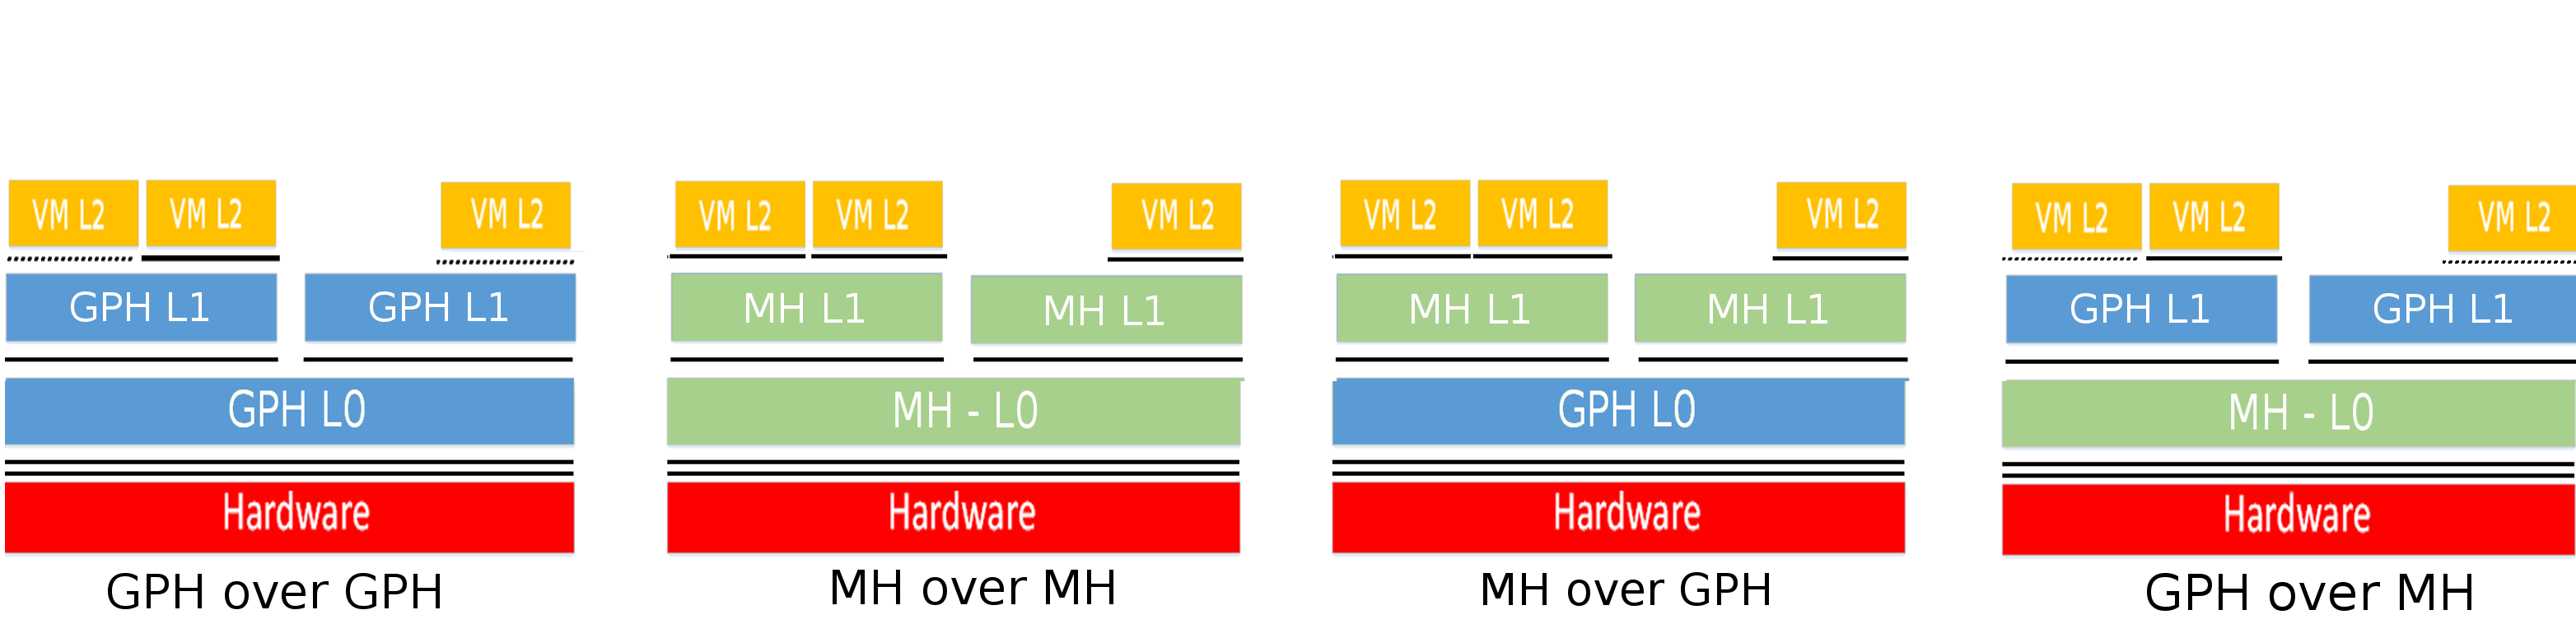
\includegraphics[width=2\columnwidth]{globalcut.png}
\end{center}
\caption{Different Types of Nested Architectures.}
\label{fig:io}
\end{figure*}

\subsection{Limitations}

\noindent The MH approach also showed several limitations. First, support for hardware is lacking, notably in terms of device drivers. Fortunately, this issue may be addressed leveraging I/O passthrough techniques, despite some resulting exclusive allocation challenges.
Second, several cloud issues are simply not addressable with GPHs. However, GPHs are now widely adopted and foundation of existing cloud platforms. While a GPH exports mature APIs to upper software layers and is also tightly integrated with cloud toolkits, MHs lack such API stability and integration, requiring explicit dedicated code to be written -- thus violating DP5.  
Third, for the sake of kernel size, MHs could lack several virtualization features commonly available on modern GPH hypervisors. For instance, XMHF does not support multiple guests. Such limitations applicable for MH architectures alone may be lifted partially or totally when applying MH design to NV architectures. 

\section{Architecture Comparison}
\label{sec:archcomp}

\begin{table*}[htbp]
\caption{Architecture Comparison.\label{fin:conf}}
\centering
\begin{tabular}{llcllll}
\toprule
Id & Functional Design Principle & Class of Requirement & GPH/GPH & MH/MH & MH/GPH & GPH/MH\\
\midrule
DP1  & User-Data Privacy               & Vertical   & $\times$      & $\checkmark$  & $\times$/$\checkmark$ & $\checkmark$ \\
DP2  & Fail-Safe modular architecture  & Vertical   & $\times$      & $\checkmark$  & $\times$ & $\checkmark$ \\
DP3  & Small TCB                       & Vertical   &  $\times$     & $\checkmark$  & $\times$ & $\checkmark$ \\
DP4  & Inter-Platform support          & Horizontal & $\checkmark$  & $\times$      & $\times$ & $\checkmark$ \\
DP5  & Compatibility with Legacy       & Horizontal & $\checkmark$  & $\times$      & $\times$ & $\checkmark$ \\
DP* & Minimal Additional Code         & --         & $\checkmark$  & $\times$      & $\checkmark$ & $\checkmark$ \\
\bottomrule
\end{tabular}
\end{table*}

\noindent Adding an extra layer of virtualization enables to introduce a wide range of new features in the IaaS infrastructure, but does not reduce the TCB size. Introducing MH design within a nested IaaS architecture could represent a new approach to improve NV benefits by overcoming such limitations. In what follows, we analyze the four possible architectures shown in Figure~\ref{fig:io} to achieve nesting of GPH and MH, highlighting their potential, and assessing their benefits and weaknesses w.r.t. to the design principles of Section~\ref{ref:challenges}, as well as their cost of implementation.

\subsection{GPH/GPH}

\noindent The first architecture only features GPHs in both layers to serve as point of comparison. This type of architecture enables several remarkable features related to VM management flexibility such as live migration over different platforms, and transparent migration of virtualized clusters across data centers, fulfilling principle DP4. More generally, assuming complete and correct support of virtualization primitives for nested hardware in mainstream hypervisors, this architecture satisfies all horizontal design principles. 

However, it fails to safisfy vertical design principles as TCB size is that of currently deployed NV architectures. The interest of other MH-based architectures will thus be to introduce isolation and privacy improvements by reducing the TCB, while still keeping horizontal features.

%Although this architectures presents an extra layer between the nested guest, normally controlled by the cloud user and the system critical part, L0, the latter is far from a satisfying security level. The TCB of KVM that is represented by the entire Linux Kernel is normally around 200 KLoCs, considering the medium size of a deployed Linux kernel.
%Moreover, default KVM configuration does not provide a transparent protection mechanism between different VMs, so that compromising one instance of QEMU, that is executed in user-space, an attacker could compromise all the others VMs on the platform.

\subsection{MH/MH}

\noindent This architecture is considered only to highlight the improvements of a MH design compared to a GPH/GPH architecture. An MH/MH implementation would meet the vertical requirements missing in the previous approach. 
As in single-layer MH architectures, hypervisor disaggregation and minimization overcomes issues posed by monolithic system architectures and over-privileged administrative VMs (DP1). The smaller resulting TCB also improves resilience of the platform against a large set of software failures (DP2) and reduces the surface of attack of the most privileged part of the IaaS infrastructure (DP3). 

However, the interest this class of architecture remains limited as it cannot overcome any of the generally cited issues of single-layer MHs such as compatibility with legacy hypervisor architectures (DP5). While several horizontal properties are theoretically achievable, they would require a large development effort to implement the relevant features such as interoperable advanced resource management. Moreover, the lack of nested VMX support prevents testing in practice this type of architecture, as MH usually rely on VMX primitives to create nested HVM guests.

Overall, with this architecture, if vertical challenges are well addressed as in single-layer MHs, it does not provide any improvement for horizontal challenges, despite NV being used to bridge gaps between IaaS platform eco-systems.

\subsection{MH/GPH}
\label{par:mog}

\noindent The third architecture aims to address security concerns. It combines a GPH as L0 and a MH as L1. 
%Several MH are proposed in literature focusing on different .
%Therefore, this model tries to exploit microhypervisor as L1 hypervisor in order to enforce better isolation between L2 and L0. L1 will exploit the emulated nested VMX provided by GPH L0 and virtualize L2. 
%With this approach, we try to isolate the attacker in a VM virtualized on a secured layer, in order to prevent attacks to L0. The attacker would have to face with an essential virtualization layer and it would not be able to attack the back-end virtualization layer. 
This approach is interesting as it may be easily deployed without requiring any extra code addition to the GPH. Hardware support is not a real barrier as existing GPH-based platforms could potentially export nested VMX features to guests. Even if this is not yet the case in modern cloud platforms, this lack may be considered temporary due to the experimental status of such features.

However, there is no TCB reduction as the code size running in L0 kernel space is as big as before. 
Besides, adopting a MH as L1 prevents using inter-platform enhanced features. As already seen for MH design, the price of having a thin hypervisor is normally paid with a lack of certain features. 
%For example, XMHF only supports a single guest~\cite{xmhf}. 
Thus, this architecture cannot provide any new horizontal features leveraging NV. Therefore, this approach can only provide the same features as those deployed today, with an increased but not sufficient level of isolation.

\subsection{GPH/MH}
\label{par:gom}

\noindent This last approach achieves a smaller TCB than other architectures, due increased modularity brought by the micro-kernel-like design of the L0 layer -- satisfying DP3. Leveraging a GPH like Xen or KVM for the L1 layer provides the user with an environment seeming identical to those used in production today -- satisfying DP5. The L1 GPH is normally integrated with modern cloud toolkits like OpenStack, and will thus support third-party applications -- satisfying DP4.
Therefore, this architecture achieves a stronger level of isolation due to vertical use of NV to introduce an additional hardware-protected security monitor. Thanks to the GPH, the MH layer remains transparent to the user and should not impact the functional properties of the IaaS platform.

This class of architecture may suffer from two types of limitations. First, nested VMX extensions must be exposed to the L1 hypervisor to let him ``nest'' another HVM guest. This requirement is implemented by GPHs like Xen and KVM, but usually not included in the key features to be provided by a MH: implementing nested VMX may be estimated to around 1KLoC, to be compared with the size of a typical MH (2-20 KLoC)~\cite{xmhf}.
More generally, the MH quest towards ever increasing minimalism could represent a serious limitation to preserving functions of existing platforms: the constraint of privileged code size may force MH developpers to drop some features considered as non-essential. This may apply to NV-related primitives, but also to other types of features. For instance, XMHF may only virtualize a single L1 instance at a time. While this may be acceptable if the platform objective to enforce strict resource access control in a single-provider private cloud, it hinders having a platform model enabling the user to run its own hypervisor as L1 to set up a self-service cloud independently from the underlying provider -- as in that case, multiple L1 hypervisors would need to run concurrently on the L0.

Second, device drivers should be correctly managed. Drivers are a major MH issue, due to costs of development or of adaptation to a new architecture. Such challenges may be addressed using device assignment: the L1 GPH hypervisor manages the physical device with the proper driver now running in a lower level of privilege. To be workable, this approach would require exclusive allocation to be simply implementable, e.g., using SR-IOV~\cite{sriov}.

\subsection{Discussion}

\noindent Overall, how do such architectures compare to the two main reported benefits of NV, i.e., vertical, through an increased level of isolation between hypervisor and customer VMs, and horizontal to easily achieve multiple provider platform interoperability at system level? Table~\ref{fin:conf} summarizes the previous analysis. 

The GPH/MH architecture appears as the most interesting to expand the NV promised benefits. Through a solid and secure MH as L0, it is the only one able to reduce the platform TCB. This would bring several benefits towards a more secure infrastructure. First, a guarantee that the platform administrator could not lose control of the system thanks to an extra security layer. Second, certification perspectives: Klein et al.~\cite{Klein:2009} showed that less than 10 KLoC kernels could be formally verified, under several conditions, which is far from be achievable today with standard GPH/GPH approach where the TCB is an order of 
magnitude bigger than MHs~\cite{nova}.

However, the effort to set up a GPH/MH is strongly dependent on the technique for L2 virtualization. As already seen, to support L2 guests with hardware-assisted virtualization which is becoming mainstream, the MH needs to export nested VMX primitives. On the other end, adopting paravirtualization or dynamic binary translation for L2 does not requires particular hardware support, and thus would not require MH patching to set up a running platform. However, paravirtualization supports only a subset of system features, which could be an issue as general solution.
%The last point of interest is related to device management. If MH act as L0 hypervisor, it has to deal with hardware devices, and this could necessitate of a significant code writing. In fact, there are several technologies, like Direct Assignment, allowing to bypass hypervisor control of a device. Those techniques are useful but they reduce the flexibility in the device management, requiring for example exclusive allocation of a device to a guest. To contrast this drawbacks, PCI-E propose the possibity to multiplex device with a set of virtual devices called virtual functions proposed to the L0 hypervisor, that will relax the contraint of exclusive allocation. Unfortunately this approach could not give the same flexibilty given by other techniques, like para-virtualization 
%With MH over GPH, MH could directly assigne devices to GPH that is able to implement  para-virtualize device, for example. 
%This will relief the MH of a part of devices management, giving to the GPH the responsibility to drive concretely the device but without losing interesting features. Therefore, we will need a limited amount of code to handle device without have to deal with each specific device.

Therefore, a MH-based architecture could increase the feature set of current NV architectures, mostly vertically. The main remaining barrier is to come up with an MH implementation supporting HAV nested guests. We are working on a GPH/MH implementation aiming to lift this limitation using paravirtualization.

\section{Towards 2D Security Management}
\label{sec:arch}

\begin{figure*}[htbp]
\begin{center}
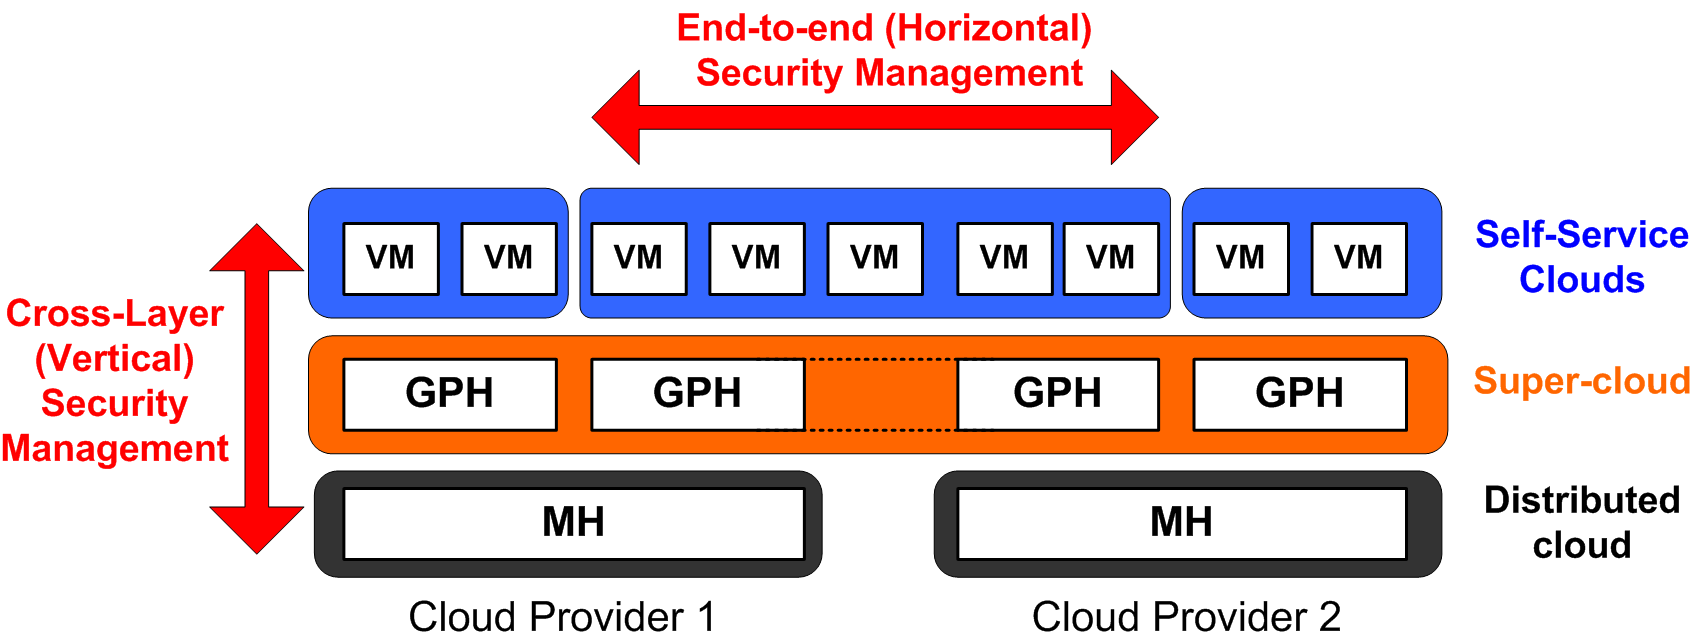
\includegraphics[width=10cm]{DCCArchitecture.png}
\vspace*{-0.5cm}
\end{center}
\caption{DCI System Architecture.}
\vspace*{-0.5cm}
\label{fig:archisecu}
\end{figure*}

\noindent We now sketch how the previous enhanced-NV design enables to build a DCI security architecture meeting both vertical and horizontal requirements. Such DCIs will face 2D threats, vertical spanning layers, and horizontal, spanning domains -- DCIs being both multi-layer and multi-domain. Vertically, attacks currently target several infrastructure layers (e.g., VMs, hypervisor). Unfortunately, most existing defenses are generally for single layers only. This makes it difficult to grasp the overall extent of an attack. Horizontally, threats may propagate through the network from cloud to cloud. Unfortunately, most existing defenses are for single clouds only. Lack of interoperability in security policies and mechanisms is thus a major barrier to  unified hybrid cloud security. Overall, DCI security requires 2D protection.

%3 Layer infrastructure
We consider the 3-layered DCI architecture shown in Figure~\ref{fig:archisecu}. The bottom and top layers are similar to a single-cloud IaaS.
\begin{itemize}
\item
%Provider:
At the bottom is the \textit{provider-centric} view of the DCI: each cloud provider contributing to the DCI is in control of compute, storage, and network resource provisioning.  
%Top User-VM
% of the cloud each provider providing layer and t
% On the top are the VM built self-service security where security is personalized/customized.
\item At the top is the \textit{user-centric} view of the DCI: customer VMs are arranged in a set of \textit{self-service clouds} (SSCs) where security and other services may be fully customized by users, independently from underlying providers.
%Middlelayer: Supercloud
\item The middle layer is a distributed resource abstraction and security management plane we call the \textit{security super-cloud}.
\end{itemize}

%Super-cloud 
%The SUPERCLOUD will fulfill that vision with a two-level infrastructure:
The super-cloud has two main functions.
% Fonction North
% Fonctions 1: SUPERCLOUD Layer built SS cloud
% implementing the self-service security to build SSChe lower part of the SUPERCLOUD is be a distributed infrastructure will realize the distribute resource abstraction layer  and . It will implement the northbound, user-centric super-cloud API.
%The northbound, user-centric super-cloud API will implement self service security and dependability, allowing to build self-service clouds (SSC) where VM, network, and storage security may be personalized independently from the underlying provider. Such clouds may be defined at the service level to the full IaaS, relationships between SSC being flat or nested, also with complex trust relationships between sets of SSC according to the ecosystem relationships of the super-cloud providers providing the SSC.
Its northbound interface federates cloud resources in a provider-independent manner and enables to customize their security to realize the SSCs. While many orchestration architectures have been proposed at service or middleware levels (e.g., multi-Iaas platforms), our architecture aims to achieve federation at system-level to fully take advantage of underlying provider platform openness (if available) for finer-grained control and increased flexibility.
% Fonction South
% Fonction  2:
% The southbound, provider-centric super-cloud API will define a unified security and dependenability management plane of the compute, data, and network resources independently from providers. This may apply for B2B use cases to management of clouds of clouds but also to device-to-cloud scenarios if devices are considered, with possible extensions to the personal cloud for device-to-device scenarios, the SSC taking the form of personal cloud-based digital infospheres where security and dependability may be totally user-controlled.
% Also security management both vertically and horizontally.
% This means: providing vertically a cross-layer integrated vision of security of the cloud and SUPERCLOUD infrastructure; defining horizontally a security abstraction layer to achieve a homogeneous level of security across clouds independently from underlying provider mechanisms; and integrating both dimensions smoothly. This approach is key to providing a unified view of security of the SUPERCLOUD.

% bove, the upper part of the SUPERCLOUD will be a supervision infrastructure providing a set of security and resilience services to guarantee the security of the overall SUPERCLOUD architecture. It will realizing self-service security, end-to-end security, and resilience. It will implement the southbound, provider-centric super-cloud API.

The super-cloud southbound interface is in charge of 2D DCI security management. It provides a unified vision of security across layers of the DCI, guarantees a homogeneous level of security across clouds independently from underlying provider mechanisms, and integrates both dimensions smoothly. 
% Automation
% Pour l'intégration: requirement: autonomous
% Automation.
%Despite some automated solutions for managing security of single clouds, there is currently no solution truly applicable to federations of clouds in practice.
% and security management complexity. Th
% 360 Atuomation
Despite many defense mechanisms being available in this 2D landscape, they remain difficult to configure and to reconcile, the current ``by hand'' approach for supervision being a nightmare for security administrators. To overcome such complexity, we consider here a security monitoring infrastructure providing 2D detection and reaction to threats with a high degree of automation.

%OS:
In terms of system architecture, we consider a NV-based design to realize the super-cloud above the DCI as in~\cite{xclo:blank}. 
%Layer 1: MH Ce que cela permet
% Provides enhanced security
% Achieve Vertical security Cross Layer security
We assume the provider-layer to be MH-based. 
This design choice provides a solid foundation to meet all vertical features, notably smaller TCB size and enhanced DCI security such as guaranteeing VM security even if intermediate layers are compromised. 
Note that this assumption does not seem unreasonable for the coming years as: 
%Provider MH: Assumption min V, XenDisagregated...
(1) despite most current IaaS platforms still being GPH-based, there is a strong trend towards making the hypervisor more minimal and flexible, as witnessed by disaggregation of hypervisors of the mainstream IaaS platforms~\cite{XOAR,MinV}; 
% Interoperability betwene differnet component-based design such as XMHF.
(2) MHs themselves are becoming component-based, with possibility of interoperability to avoid any further risk of IaaS lock-in as shown by first multi-MH  OS frameworks~\cite{xmhf}. 
% Above GPH: 
% 
% GPH allows also to layer of interoperability horizontal blanket layer above the different MH to enalbe self-service security.
% Layer 2: GPH Ce que cela permet. Verticalement et horizontalement.
% % Blanket layer .

The super-cloud layer is GPH-based, both to be able to realize the SSCs by defining blanket layers and to guarantee security interoperability and other horizontal features. 

%Framework VESPA horizontal UCC
% Cross-Domain Framework:
% ou VERTICAL ICAC.
% Cross-Layer Framewokr: VESPA
To implement 2D security management proper, we intend to rely on self-protection frameworks which have been defined for both cross-layer~\cite{VESPA} and cross-domain~\cite{VESPA:UCC} IaaS and multi-IaaS integrated security monitoring. We are currently investigating how they may be integrated within the previous system architecture, notably to guarantee security SLAs~\cite{CUMULUS}.


%The SUPERCLOUD project aims to define the architecture and build the infrastructure to fulfill the vision of user-centric secure and dependable management of a clouds of clouds. Our approach will be to define a new distributed architectural plane, the super-cloud providing an end-to-end interface both between user-centric and provider-centric views of multiple clouds. Its role will be both to provide a distributed resource abstraction and flexible but unified control for management of security and resilience.
%From the user perspective, the super-cloud will enable user-centric security and dependability through a unified distribution layer for cloud resources, independently from their type (computation, storage, and network) and from underlying cloud providers. It thus forms an intermediation layer for resources between their production by providers and their consumption by users. This in line with the vision introduced by IBM [X] as well as with the utility computing paradigm [X], but will go well beyond, leveraging this distribution layer to explore high customizability of user cloud security and dependability according to well-defined SLAs. 
%From the provider perspective, the super-cloud will also enable provider-independent control over security and resilience over the overall distributed cloud infrastructure, security being autonomous managed and guaranteed end-to-end. This will also make the resource distribution layer both secure and resilient. 
%The level of abstraction, from system to middleware interoperability of the super-cloud be also be tuned to allow trade-offs between user-centric and provider-centric control for security services. 
%In terms of architecture:
%The northbound, user-centric super-cloud API will implement self service security and dependability, allowing to build self-service clouds (SSC) where VM, network, and storage security may be personalized independently from the underlying provider. Such clouds may be defined at the service level to the full IaaS, relationships between SSC being flat or nested, also with complex trust relationships between sets of SSC according to the ecosystem relationships of the super-cloud providers providing the SSC. 
%The southbound, provider-centric super-cloud API will define a unified security and dependenability management plane of the compute, data, and network resources independently from providers. This may apply for B2B use cases to management of clouds of clouds but also to device-to-cloud scenarios if devices are considered, with possible extensions to the personal cloud for device-to-device scenarios, the SSC taking the form of personal cloud-based digital infospheres where security and dependability may be totally user-controlled.
%...
%The SUPERCLOUD will fulfill that vision with a two-level infrastructure:
%•	The lower part of the SUPERCLOUD is be a distributed infrastructure will realize the distribute resource abstraction layer federating distributed cloud resources and implementing the self-service security to build SSC. It will implement the northbound, user-centric super-cloud API.
%•	Above, the upper part of the SUPERCLOUD will be a supervision infrastructure providing a set of security and resilience services to guarantee the security of the overall SUPERCLOUD architecture. It will realizing self-service security, end-to-end security, and resilience. It will implement the southbound, provider-centric super-cloud API.
%In what follows, we describe the SUPECLOUD vision for each self-service security, self-managed security, end-to-end security and resilience properties. 
%
%For computing workloads, user-centric cloud security management faces two challenges.
%•	Lack of IaaS infrastructure openness: provider-controlled immutable hypervisors (or that mask access to the hardware) prevent users from taking advantage of hypervisor-level advanced resource management and security services such as high availability or VM introspection for fine-grained VM misbehavior detection and reaction. Such examples of vendor lock-in are already a notorious issue for single provider infrastructures [CSA Guidance]. They are a real barrier for hybrid clouds: the varying degree of openness of the underlying IaaS forces to achieve security interoperability in upper software layers instead of at system level as in multi-IaaS orchestration platforms, highly reducing user control over security management. Such limitations also prevent fine-grained trade-offs between provider and user control over security : among security services, users cannot choose between those to customize, and those to delegate to the provider infrastructure.
%•	Security threats for customer VMs: large, complex, overprivileged hypervisors are a serious risk for VMs [CSATT]. The assumption of a trusted hypervisor is no more, illustrated through many examples of VM escapes, breaking hypervisor isolation through exploitaiton of device drivers vulnerabilities [Virtunoid, CloudBurst]. A multi-layer approach to IaaS security is needed considering lower layers, to guarantee VM security even if the hypervisor layer is compromised. This challenge is intrisically linked with openness and flexibility issues: from a user perspective, to protect their VMs from an untrusted provider infrastructure, customers may wish adding their own security modules (or layer) in the infrastructure, provided it is open enough. Conversely, a provider may also wish to benefit from an open hypervisor architecture to harden its IaaS against rogue VM behaviors.
%Earlier IaaS architectures such as disaggregated hypervisors or nested virtualization provided partial answers to either of those issues but not both. Hypervisor disaggregation (for the Dom0 or the core hypervisor) achieves flexibility through the definition of clearly separated access control domains between provider-centric and user-centric security management planes where fine-grained trade-offs may be reached [SSC]. This approach is compatible with legacy hypervisors (Dom0 case) or requires new architectures (core hypervisor case). However, it only addresses security and flexibility challenges in a single cloud context, but not for interoperability of multiple independent hypervisors. Nested virtualization addresses the (vertical) security challenge by placing an additional hardware-protected security monitor beneath the untrusted virtualization layer [Turtles, CloudVisor] -- requiring a sufficiently open IaaS. It also features (horizontal) flexibility and interoperability benefits by defining a blanket layer on top of existing provider hypervisors in a hybrid cloud setting, enabler for self-service security for clouds of clouds [XenBlanket]. However, such horizontal and vertical benefits have not yet been combined in a unified security architecture. Moreover, the additional layer separation might also make user vs. provider trade-offs more coarse-grained than the previous approach.
%Hence, in SUPERCLOUD, we propose to define a new IaaS security architecture for distributed clouds that may combine the benefits of the two previous architectural approaches in terms of both layered design and modularity to achieve self-service cloud security with tuneable, fine-grained trade-offs with provider-centric security to protect customer VMs. The benefits of this hybrid approach will be to lift both barriers simultaneously, but also to be applicable in a large variety of underlying provider infrastructures. For instance, if the underlying hypervisor is not open, leveraging the benefits of nested virtualization for hypervisor interoperability; and otherwise, using either approach, depending on desired security vs. performance trade-offs, and compatibility with legacy systems or deployment of new security hardened IaaS architectures.
%
%

%
%%
%%%%Improving the Status Quo
%Udo Steinberg NOVA 6
%Virtualization layer is critical. Make it as small as possible.
%Design Principles:
%1)Fine-grained functional decomposition
% Microhypervisor (privileged)
% Multiple user-level VMMs (unprivileged)
% User-level drivers, applications (unprivileged)
%2)Principle of least privilege among all components
% Capability-based authorization model
%Ideas adopted from the microkernel world
%Those still existing limitations to nested HVM, made we focus on nested PV.
%Leveraging on the new architecture presented we propose a security architecture based on Xen and NOVA. 
%
%Xen is a well-known and wide-used hypervisor that is the base of several of most important cloud platforms.  We focus in particularly on the Xen support for para-virtualization. 
%
%Available from the first version of Xen in 2003, PV does not requires any specific hardware facilities. Even if some features drop in Amd64 architecture leaded to a little performance loss for PV compared to HVM guests, the real limit of PV is represented by the impossibility to virtualize Windows and other proprietary operating systems.
%However this technique is currently still exploited in widespread cloud platform like Amazon EC2.
%
%NOVA is a tiny micro-hypervisor able to virtualize several guests. It is a recent but promising open-source project developed at Technische Universitat Dresden. The aim of project is double: minimize the amount of code running in kernel mode and try boost virtualization.
%
%NOVA implements some interesting features, in particular from security point of view. It adopts a capability-based authorization model in order to implement the principle of least privilege among components. It supports SMP guests, VT-d Direct device assignement and NPT/EPT.
%
%The modular architecture of NOVA allows also to enforce a increased separation between different L1 guest. Leveraging the modular architecture of NOVA, each L1 guest communicates directly with a separate instance of the Virtual Machine Monitor, component of the hypervisor executed in user space. 
%
%The concept is to boot and use Xen as L1 hypervisor, inside a NOVA VMs. Xen hypervisor will be able to virtualize complete PV guests in a secured Cloud Platform. The presence of NOVA is completely transparent for the user.  

%Therefore, leveraging NOVA as L0 our platform could propose inter-platform features to the user. We have the opportunity to exploit a complete cloud toolkit with the Xen hypervisor implementing features like inter-platform migration and improved redundancy, as described in the Xen Blanket approach.

\section{Conclusion and Future Work}
\label{sec:conclu}

\noindent This paper reviewed the main DCI design challenges and how they could be addressed by combining NV with different hypervisor architectures. We also presented a preliminary system architecture combining GPHs and MHs for 2D security management of DCIs. 

Ongoing work focuses on refining this architecture to add self-protection features based on the VESPA framework. The objective is to determine where to place detection, decision, and reaction components for the different autonomic security loops, both within layers and across clouds. We are also implementing a proof-of-concept prototype of this security architecture using Xen as L1 GPH and NOVA as L0 MH. Xen seemed the most suitable hypervisor for L1, notably due to its support of different virtualization techniques and ability to run without HAV support. NOVA appears promising for L0 due to its clean design and code availability. With this platform, we are currently focusing on implementing vertical properties (e.g., cross-layer self-protection) in a single cloud setting, with extension to horizontal properties (e.g., inter-cloud self-protection) in a distributed cloud setting.

%On the other hand, L1 choice is much simpler. 
%
%, focusing first on vertical properties in a single cloud setting, and extending it to horizontal properties in a distributed setting.
%
%
%\begin{itemize}[]
%\item \textbf{Inter-platform support} Executed as L1, Xen would virtualize its nested guest initially using PV delivering the compatibility layer.
%\item \textbf{Tiny TCB} The NOVA kernel will represent the only part of the platform executed at the highest level of privilege. Even the VMM, Vancouver, will be executed in the L0 user-space. The micro-kernel in L0 enforces a strictly modular approach to L0. Therefore, the VMM will present distinct processes instances for each L1 guest, enforcing a context division.
%\item \textbf{3rd part compatibility} From a user point of view the architecture still exports the same interfaces provided by the Xen hypervisor, allowing the user to keep its applications unchanged.
%\item \textbf{Fail-safe components architecture} Moreover, the tiny core is the only safety-critical software component. The system could potentially be able to recover any crash in different user-space components.
%\end{itemize}
%
 %
%
%After this initial study, the first step will be deploying a minimal nested architecture testing ``out-of-the-box'' features and limitations. The following part will concern the conception of patch and extensions in order to adapt the general design of MH to properly act as L0.
%The final goal is to provide an architecture able to leverage nested virtualization cloud platforms improvements, having a smaller TCB and allowing customers to leverage flexible migrations and scheduling.

%
% Our vision is that the security of the SUPERCLOUD should be both self-managed and 360.

% Our ambition is to define a security supervision architecture and framework for the SUPERCLOUD enabling this 360 view of security management with a high level of automation. Thus, the SUPERCLOUD will bring unified, simple management of security for cloud of clouds.


%In the previous sections we proposed a functional analysis of cloud architecture in order to respect design principles that we identified in the introduction. In this section, we propose a GPH over MH implementation, based on .
%
%\begin{itemize}[]
%\item \textbf{Inter-platform support} Executed as L1, Xen would virtualize its nested guest initially using PV delivering the compatibility layer.
%\item \textbf{Tiny TCB} The NOVA kernel will represent the only part of the platform executed at the highest level of privilege. Even the VMM, Vancouver, will be executed in the L0 user-space. The micro-kernel in L0 enforces a strictly modular approach to L0. Therefore, the VMM will present distinct processes instances for each L1 guest, enforcing a context division.
%\item \textbf{3rd part compatibility} From a user point of view the architecture still exports the same interfaces provided by the Xen hypervisor, allowing the user to keep its applications unchanged.
%\item \textbf{Fail-safe components architecture} Moreover, the tiny core is the only safety-critical software component. The system could potentially be able to recover any crash in different user-space components.
%\end{itemize}

%On the other hand, L1 choice is much simpler. Previous analysis identified Xen as the most suitable hypervisor for this role. The capacity to support different virtualization techniques added to the ability of running without HV support, makes Xen suitable to act as compatibility layer. 
%
%After this initial study, the first step will be deploying a minimal nested architecture testing ``out-of-the-box'' features and limitations. The following part will concern the conception of patch and extensions in order to adapt the general design of MH to properly act as L0.
%The final goal is to provide an architecture able to leverage nested virtualization cloud platforms improvements, having a smaller TCB and allowing customers to leverage flexible migrations and scheduling.


%\section{Conclusion}
%{\scriptsize
%\bibliographystyle{abbrv}
%\bibliography{biblio}
%}

{\scriptsize
\bibliographystyle{abbrv}
\bibliography{biblio}
}
\end{document}
